In this chapter the sensors for the drone will be chosen, so they will fulfill the requirements given for the sensors. To make this choice some different Time-of-Flight sensors will be examined.
\section{Time of Flight sensors}\label{s:sensor_choice}
A ToF sensor works by sending out a signal, and timing the delay before the reflection of this signal is received. In the section \ref{s:navi} (Navigation) the different types of ToF sensors have been examined, and in that section it have been chosen that the sensor that suit this project most will be ether a IR sensor or a ultrasonic sensor. From these sensor types the following sensors have been chosen to be looked through:
\begin{itemize}
    \item IR
    \begin{itemize}
        \item VL53L0X %%%%
        \item VL53L1X 
    \end{itemize}
    \item Ultrasonic
    \begin{itemize}
        \item CH-101
        \item CH-201
        \item HC-SR04
    \end{itemize}
\end{itemize}
From this list of of sensors, it have been chosen that the sensor suited best for this project is the VL53L0X, which fulfill the requirements for what the sensors.

\section{Setup of the sensor}\label{setup_sensor}
Before setting up the sensor to the drone, some technical information is needed to have knowledge of these sensors.
First the geometric of the sensor is shown in figure \ref{fig:sensor_geometric}, here is both for the transmitting led and the receiving led. The funnel from each of the leds is the field the sensor can transmit to and receive from. The small led is the transmitter and the big one is the receiver. 
AS told before, the sensor works by sending out a IR signal and times the time used before it receives the reflected signal again.
\begin{figure}[H]
    \centering
    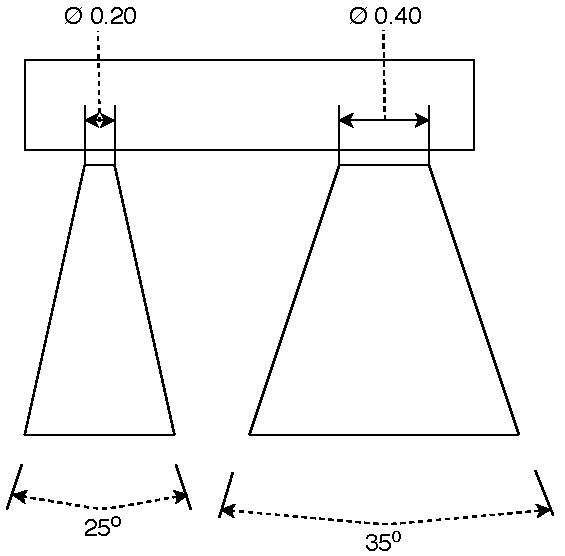
\includegraphics[width=0.6\textwidth]{figures/ch_design/Sensor.pdf}
    \caption{Caption}
    \label{fig:sensor_geometric}
\end{figure}
The sensors communicate with a micro controller using i2C, which means it use the pipelines SCL and SDA. The sensors have different modes it works in default mode, high accuracy, long range and high speed. The four modes can be seen in the tabular \ref{tab:sensor_mode}, here both the refresh time and maximum distance for each mode are noted. 
\begin{table}[H]
\caption{Sensor modes}\label{tab:sensor_mode}
\begin{tabular}{|l|l|l|}
\hline
\textbf{Mode}          & \textbf{Refresh time} & \textbf{Maximum distance} \\ \hline
Default mode  & 30 ms        & 1.2 m            \\ \hline
High accuracy & 200 ms       & 1.2 m            \\ \hline
Long range    & 33 ms        & 2 m              \\ \hline
High speed    & 20 ms        & 1.2 m            \\ \hline
\end{tabular}
\end{table}
The most suited mode for this project will be the high speed mode, by using this mode the refresh time is faster than the required frequency at 40 Hz.  

\section{Test of sensors}
To see if the VL53L0X sensors are complying ti the requirements from the chapter \ref{ch:Req}. A test have been preformed to determine if the they meet the requirements . The full test of the sensors can be seen in appendix \ref{ap:testOfSensors}. The requirements that the sensors have been tested against are the following:
\begin{itemize}
    \item Detect a surface from minimum 1 meter.
    \item Accuracy of $\pm$5 \% at 400 mm.
    \item sampling rate of 40 Hz
    \item detection of wall with a angle of 0$\degree$ $\pm 10 \degree$
\end{itemize}
The test have been preformed with the sensors mounted on an Arduino with a breakout board faced against a white wall. The code used to test can be found on the Github repository \url{https://github.com/AAU-EIT5/VL53L0X-sensor-test}. 
\newline
\newline
The results of the test can be seen in the figures \ref{fig:des_Sensor1TestResult} and \ref{fig:des_Sensor2TestResult}.
\begin{figure}[H]
    \centering
    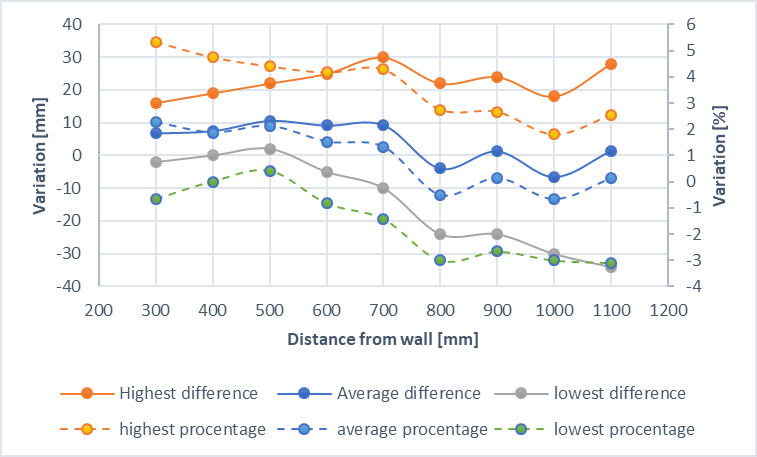
\includegraphics[width=0.8\textwidth]{figures/Appendix/resultatSensor1Test.png}
    \caption{Result of sensor 1 for the test.}
    \label{fig:des_Sensor1TestResult}
\end{figure}
\begin{figure}[H]
    \centering
    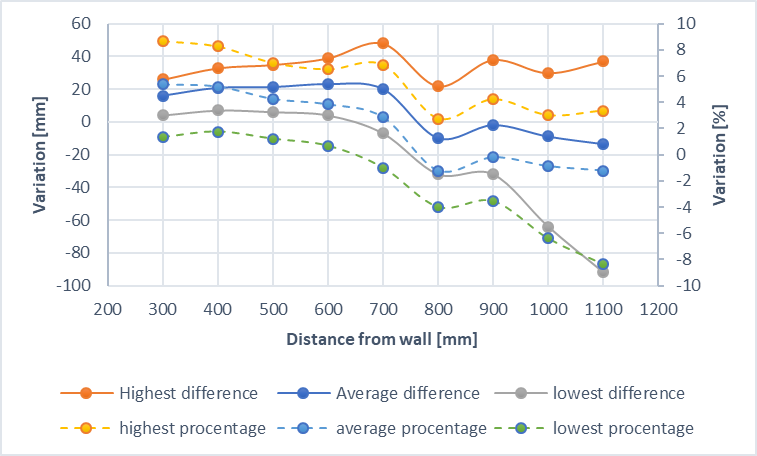
\includegraphics[width=0.8\textwidth]{figures/Appendix/resultatSensor2Test.png}
    \caption{Result of sensor 2 for the test.}
    \label{fig:des_Sensor2TestResult}
\end{figure}
From these results the first requirement of detection of a surface at lest 1 meter can be confirmed. As it can be seen on figure \ref{fig:des_Sensor1TestResult} and \ref{fig:des_Sensor2TestResult}, that both sensors can detected a surface at a distance of at lest 1.1 meter.
\newline
From the figures the second requirement of $\pm5 \%$ accuracy at 400 mm distance can also be confirmed. as it can be seen on the figures the lowest accuracy of the sensors around $\pm 4 \%$ at 400 mm, if the displacement of the sensors measured distance from the real into consideration. As the accuracy are within the requirements, the requirement can be seen as fulfilled.
\newline
As the test was running, a timer was started to measure how long time it takes to complied one set of data, and a sampling rate can be found from these times. The found sampling rate of the sensors are 54 Hz, as the required sampling rate have to be at lest 40 Hz the requirement are meet.
\newline
To test the last requirement, which is to detect a surface at a angle of  $\pm 10 \degree$. This test has performed by placing the sensors 1100 mm from the wall and see if it could detect the wall. The angle is set to $10 \degree$ both for the right and left direction. The result of the test shows that the sensor still is possible to detect a wall. From this test it is therefor conclude that the sensors fulfill the requirements for the sensors.

%
%
%
\section{Interfacing with the sensors}\label{sec:interfacingVL53L0X}%find en bedre overskrift
When using the sensor VL53L0X it's necessary to interfacing with it, to do this the library VL53L0X from Pololu will be used. 
\newline
To start, the address of the sensor have to be setup, this are done by the \textbf{\textit{setaddress()}} function. After setting the address the sensors is initialized with the function \textbf{\textit{init()}}. To change the time the sensors have to measure the distance, the function \textbf{\textit{setMeasurementTimingBudget(uint32{\_}t budget{\_}us)}}, where the  \textbf{\textit{budget{\_}us}} are the time in microseconds.
To start the measuring continuously the function \textbf{\textit{startContinuous()}} is used, and with this the setup of the sensors is done.
To get a measuring in continuous mode the function \textbf{\textit{readRangeContinuousMillimeters(void)}} is used.

%As mentioned earlier in section \ref{setup_sensor} the VL53L0X sensors uses i2C at the communication method 
% her skal der stå hvordan sensorne settes op så værdier kan læses.